\section{Problema 2: Caballos salvajes}

\subsection{Introducci\'on}
La misma empresa nacional del anterior problema ahora quiere incursionar en el negocio de los juegos de mesa, por ello han sacado un innovador juego que utiliza un tablero cuadrado de ajedrez (hay en distintos tamaños) en donde se colocan en algunas casillas caballos blancos de ajedrez. El juego permite que haya mas de un caballo en la misma casilla, y los caballos pueden moverse por el tablero como lo harían en el ajedrez. Para ganar el juego hay que lograr ubicar a todos los caballos en una misma casilla en la menor cantidad total de movimientos posibles, es decir que la suma de los movimientos de todos los caballos en el tablero sea la menor. \\
A continuación se muestra un ejemplo del juego con su respectiva solución: \\

%\begin{figure}[h]
%  \centering
%    \includegraphics[scale=5]{Imagenes/introCaballos}
%  \caption{}
%  \label{fig:ejemplo}
%\end{figure}
%
%
%\begin{figure}[h]
%  \centering
%    \includegraphics[scale=5]{Imagenes/introSolu}
%  \caption{}
%  \label{fig:ejemplo}
%\end{figure}

\begin{figure}[H]
  \centering
		\begin{subfigure}[b]{0.3\textwidth}
                \includegraphics[scale=3]{Imagenes/Ej2/introCaballos}
                \caption{Inicio del juego}
                \label{fig:intro}
        \end{subfigure} 
  		\begin{subfigure}[b]{0.3\textwidth}
               \includegraphics[scale=3]{Imagenes/Ej2/introSolu}
                \caption{Solucion al juego}
                \label{fig:intro}
        \end{subfigure}
        \caption{Aunque no es visible en (b) se encuentran los dos caballos en el mismo casillero} 
\end{figure}


\subsection{Desarrollo}

Este problema lo resolvimos con una serie de pasos, primero comenzamos representando el tablero con el siguiente grafo: \\
Sea G(V,E) el grafo donde cada nodo v $\epsilon$ V representa una casilla del tablero y dos nodos $v_1$ y $v_2$ $\epsilon$ V están unidos por una arista e $\epsilon$ E $\Leftrightarrow$ es posible mover al caballo de la casilla $v_1$ a la casilla $v_2$. \\
Luego para cada caballo en su correspondiente casilla utilizamos el algoritmo de BFS sobre G, el cual para grafos con aristas no pesadas o de igual peso nos da el camino mínimo desde un nodo origen hasta cada uno del resto de los nodos del grafo \footnote{Cormen, T.,Leiserson, C.,Rivest,R.,Stein, C.,"Introduction to Algorithms", third edition, pagina 594}. Al algoritmo de BFS lo modificamos para que a medida que busca el camino mínimo a cada casilla calcule la cantidad de movimientos que le toma llegar a ésta casilla. \\
Después sumamos lo que le cuesta a cada caballo llegar a cada casilla obteniendo el total de movimientos que cuesta que todos los caballos lleguen a cada casilla. Finalmente nos quedamos con la casilla que lleguen todos los caballos y que haya resultado con menor cantidad total de movimientos. En caso que no haya ninguna casilla tal que todos los caballos lleguen a esta entonces la solución al problema será "no".



\begin{codebox}
\Procname{\textbf{Pseudoc\'odigo:}}
\li	creamos una matriz $acumMovimientos$ inicializada en 0
\li	creamos una matriz $cantidad$ inicializada en 0
\li	
\li	para cada caballo 
\li \ \ \	mientras recorremos G usando BFS desde la casilla donde se encuentra ubicado
\li	\ \ \ \ \ \		cantMov $\leftarrow$ contamos la cantidad de movimientos a cada casilla
\li	\ \ \ \ \ \		acumulamos en $acumMovimientos$ lo que contamos con cantMov
\li \ \ \	fin mientras
\li \ \ \	para cada casilla
\li	\ \ \ \ \ \		acumulamos en $cantidad$ si el caballo paso por esa casilla
\li \ \ \	fin para
\li	fin para
\li	
\li	buscar en $acumMovimientos$ la casilla que tenga menor cantidad de movimientos y que en $cantidad$
\li hayan pasado todos los caballos, retornar la casilla y la cantidad de movimientos
\li 
\li En caso que no existe tal casilla retornar "no"
\end{codebox}




\subsection{Demostraci\'on de correctitud} 

Antes que nada como nuestro algoritmo usa BFS, veamos que es correcto. Esto es cierto, ya que esta demostrado en el "Cormen" \footnote{Cormen, T.,Leiserson, C.,Rivest,R.,Stein, C.,"Introduction to Algorithms", third edition, pagina 594}. \\



Ahora para demostrar la correctitud de nuestro algoritmo vamos a usar inducción en n = cantidad de caballos. \\ \\

\textbf{Caso Base:} Queremos ver que nuestro algoritmo es correcto, es decir que nos da la solución óptima para 1 caballo, esto es fácil de ver pues el algoritmo aplicara BFS para calcular la cantidad de movimientos que le cuesta llegar al caballo a cada una de las casillas, y estos cálculos los guardara en la matriz $acumMovimientos$. Luego buscara en $acumMovimientos$ la casilla con menor cantidad de movimientos y se encontrara con que la casilla donde comenzó el caballo cuesta 0 (ya que no se movería) y devolvería esta casilla que costo 0 movimientos como resultado.\\

\textbf{Paso inductivo:} P(n) = nuestro algoritmo calcula correctamente en una matriz, para cada posición si llegan los n caballos y la cantidad de movimientos totales de los n caballos para llegar a tal posición.
Queremos ver que vale P(n+1), esto quiere decir que queremos ver que para n+1 caballos el algoritmo nos calcula correctamente la matriz con la cantidad de movimientos totales de cada casilla y la cantidad de caballos que pasan por cada casilla. \\

Por hipótesis inductiva vale P(n), veamos qué pasa cuando agregamos el n+1 caballo, el algoritmo recorrerá G (definido en la sección 2.2) usando BFS y para cada casilla contara la cantidad de movimientos. Una vez terminado el recorrido de BFS, se recorrerá el tablero para saber a qué casillas llega y la cantidad de movimientos a la casilla del n+1 caballo acumulando esto en lo que ya se tenía para los n caballos anteriores. Con esto terminaremos teniendo en una matriz el costo total de movimientos para cada casilla de los n+1 caballos y la cantidad de caballos que pasan por cada casilla, que es lo queríamos pues solo falta buscar la casilla donde hayan llegado todos los caballos y el costo total sea mínimo.






\newpage
\subsection{Complejidad}

A continuación el extracto más importante del código para analizar la complejidad: 

\begin{codebox}
\Procname{$\proc{\textbf{Caballos Salvajes}}$()}
\li matriz\_t acumMovimientos(n\_, vector$<$int$>$(n\_, 0)); 	\RComment{O(n$^{2}$)}
\li	matriz\_t cantidad(n\_, vector$<$int$>$(n\_, 0));			\RComment{O(n$^{2}$)}
\li	
\li	for(int cab = 0; cab $<$ k\_; ++cab) \{						\RComment{O(k*n$^{2}$)}
\li \ \ \		matriz\_t movimientos(n\_, vector$<$int$>$(n\_, 0));	\RComment{O(n$^{2}$)}
\li	\ \ \		bfs(caballos\_[cab], movimientos);				\RComment{O(n$^{2}$)}
\li
\li	\ \ \		for (int i = 0; i $<$ n\_; ++i) \{				\RComment{O(n$^{2}$)}
\li	\ \ \ \ \ \		for (int j = 0; j $<$ n\_; ++j) \{			\RComment{O(n)}
\li	\ \ \ \ \ \ \ \ \		acumMovimientos[i][j] += movimientos[i][j];	\RComment{O(1)}
\li	\ \ \ \ \ \ \ \ \		if (movimientos[i][j] $>$ 0) \{		\RComment{O(1)}
\li	\ \ \ \ \ \ \ \ \ \ \ \			++cantidad[i][j];			\RComment{O(1)}
\li	\ \ \ \ \ \ \ \ \		\} else \{
\li	\ \ \ \ \ \ \ \ \ \ \ \		if ( (caballos\_[cab].first-1 == i) \&\& (caballos\_[cab].second-1 == j)) \{								\RComment{O(1)}
\li	\ \ \ \ \ \ \ \ \ \ \ \ \ \ \		++cantidad[i][j];		\RComment{O(1)}
\li	\ \ \ \ \ \ \ \ \ \ \ \		\}
\li	\ \ \ \ \ \ \ \ \		\}
\li	\ \ \ \ \ \			\}
\li	\ \ \			\}
\li
\li	m\_ = numeric\_limits$<$int$>$::max();						\RComment{O(1)}
\li	for (int i = 0; i $<$ n\_; ++i) \{							\RComment{O(n$^{2}$)}
\li \ \ \	for (int j = 0; j $<$ n\_; ++j) \{					\RComment{O(n)}
\li	\ \ \ \ \ \	if (cantidad[i][j] == k\_) \{					\RComment{O(1)}
\li	\ \ \ \ \ \ \ \ \	m\_ = acumMovimientos[i][j];			\RComment{O(1)}
\li	\ \ \ \ \ \ \ \ \	f\_ = i+1;								\RComment{O(1)}
\li	\ \ \ \ \ \ \ \ \	c\_ = j+1;								\RComment{O(1)}
\li	\ \ \ \ \ \ 	\}
\li \ \ \		\}
\li			\}
\end{codebox}


Podemos ver que comienza creando 2 matrices de dimensiones n*n (líneas 1 y 2), lo cual demandara esa cantidad de operaciones O(n$^{2}$). Después hay un for (línea 4) que itera k veces y en cada iteración tiene que:

 \begin{itemize}
 \item	crear la matriz $movimientos$ (línea 5) de dimensión n*n $\rightarrow$ O(n$^{2}$)
 \item  BFS (línea 6) que cuesta O(n$^{2}$)
 \item  un for (línea 8) que iteran n veces, y en cada iteración tiene otro for (línea 9) que también itera n veces, y este en cada iteración hace asignaciones y comparaciones (líneas 10 a 15) que cuestan O(1). Entonces el for de la línea 8 tiene costo O(n*n*1) = O(n$^{2}$)
 \end{itemize}
 
Por lo tanto el costo del for de la línea 4 es O(k*(n*n + n*n + n*n)) = O(k*3*n$^{2}$) = O(k*n$^{2}$). \\

Luego tenemos la asignación de la línea 21 que es O(1) y el for de la línea 22 que itera n veces, y en cada iteración tiene el for de la línea 23 que tambien itera n veces, éste en cada iteración hace asignaciones y comparaciones (líneas 24 a 27) que cuestan O(1), así que el for de la línea 22 cuesta O(n*n*1) = O(n$^{2}$).\\

Finalmente el costo del algoritmo es de O(k*n*n + 1 + n*n) = O(k*n$^{2}$).
Ahora corroboremos que la complejidad de nuestra implementación de BFS es la mencionada:



\begin{codebox}
\Procname{$\proc{\textbf{bfs}}$ (coord\_t origen, matriz\_t \&m)}
\li		queue$<$coord\_t$>$ cola;								\RComment{O(1)}
\li		vector$<$bool$>$ aux(n\_, false);						\RComment{O(n)}
\li		vector$<$vector$<$bool $>$ $>$ visitados(n\_, aux);		\RComment{O(n$^{2}$)}
\li		cola.push(origen);										\RComment{O(1)}
\li		visitados[origen.first-1][origen.second-1] = true;		\RComment{O(1)}
\li		
\li		while(!cola.empty()) \{									\RComment{O(1)}
\li \ \ \	coord\_t cab = cola.front(); cola.pop();			\RComment{O(1)}
\li \ \ \	list$<$coord\_t$>$ adyacentes;						\RComment{O(1)}
\li \ \ \	dameAdyacentes(cab, adyacentes);					\RComment{O(1)}
\li		
\li \ \ \	for(auto \&v: adyacentes) \{						\RComment{O(1)}
\li	\ \ \ \ \ \		if (visitados[v.first-1][v.second-1] == false) \{	\RComment{O(1)}
\li	\ \ \ \ \ \ \ \ \	visitados[v.first-1][v.second-1] = true; \RComment{O(1)}
\li	\ \ \ \ \ \ \ \ \	m[v.first-1][v.second-1] = m[cab.first-1][cab.second-1] + 1;	\RComment{O(1)}
\li	\ \ \ \ \ \ \ \ \	cola.push(v);							\RComment{O(1)}
\li	\ \ \ \ \ \		\}
\li \ \ \		\}
\li			\}
\end{codebox}

Comienza creando la cola que es O(1), también creando 2 vectores uno de dimensión n y otro n*n, que cuesta O(n) y O(n$^{2}$) respectivamente.\\

Meter una coordenada en la cola y la asignación de la línea 5 cuestan O(1).\\

Luego tenemos un while (línea 7) que comprueba si la cola esta vacía lo que demanda tiempo constante y en cada iteración hace: 

\begin{itemize}
	\item  saca la siguiente coordenada de la cola y crea una lista de coordenadas (líneas 8 y 9) que cuestan O(1)
	\item  la función dameAdyacentes (línea 10) cuesta O(1) pues son comparaciones y asignaciones (el codigo se encuentra en "TP2/ej2/solucion.h"
	\item  por ultimo un for (línea 12) que itera sobre la cantidad de coordenadas de $adyacentes$, que a lo sumo son 8 pues son las casillas a las que se pueden llegar con los movimientos de un caballo. En cada iteración hace comparaciones, asignaciones y meter una coordenada en la cola (líneas 13 a 16) que son O(1). Por lo tanto el for cuesta O(8*1) = O(1).
\end{itemize}

Entonces el while tiene costo de O(1). y el algoritmo cuesta O(n$^{2}$).








\subsection{Testing}

Testeamos los siguientes casos de interés:
\begin{itemize}
	\item Tablero de 4*4 con 5 caballos en distintas casillas
	\item Tablero cualquiera con todos los caballos en la misma casilla
	\item Instancia generada aleatoriamente
\end{itemize}


Los test se pueden ver en el archivo: "TP2/ej2/src/tester.cpp"



\subsection{Experimentación}
Una vez hecho el análisis de la complejidad teórica, realizamos experimentos con el fin de contrastar los resultados empíricos y comprobar que el algoritmo implementado efectivamente tendrá una complejidad temporal de O(k*n$^{2}$).\\
Para los siguientes experimentos para cada caballo se toman dos distribuciones discretas uniforme entre 1 y 100 que se utilizan como valor para la posición de cada caballo.

Para el primer experimento vamos a variar la cantidad de caballos y dejar fijo el tamaño del tablero en n=100. Para reducir los posibles errores de medición y evitar que los resultados se vean alterados por entradas de peor o mejor caso sesgando los resultados, se decidió tomar una cantidad fija de 220 instancias generadas de la forma antes descrita para cada n y k. En el siguiente grafico se pueden observar los resultados:



%A continuación haremos una comparación a nivel tiempo de ejecución del algoritmo. 


\begin{figure}[H]
                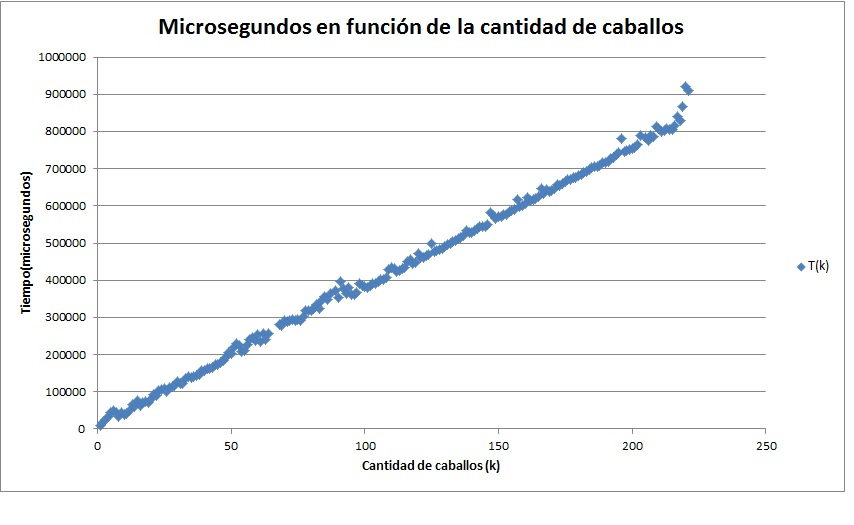
\includegraphics[scale=1]{Imagenes/Ej2/nFijo}
                \caption{T(k)=tiempo para k caballos }
                \label{fig:exp1}
\end{figure} 

Como podemos ver, obtuvimos una recta lo cual concluye al dejar constante n que la complejidad es O(k).\\

Veamos qué pasa cuando dejamos fija la cantidad de caballos en k=20 y variamos el tamaño del tablero (n) con una cantidad de 200 instancias:

\begin{figure}[H]
                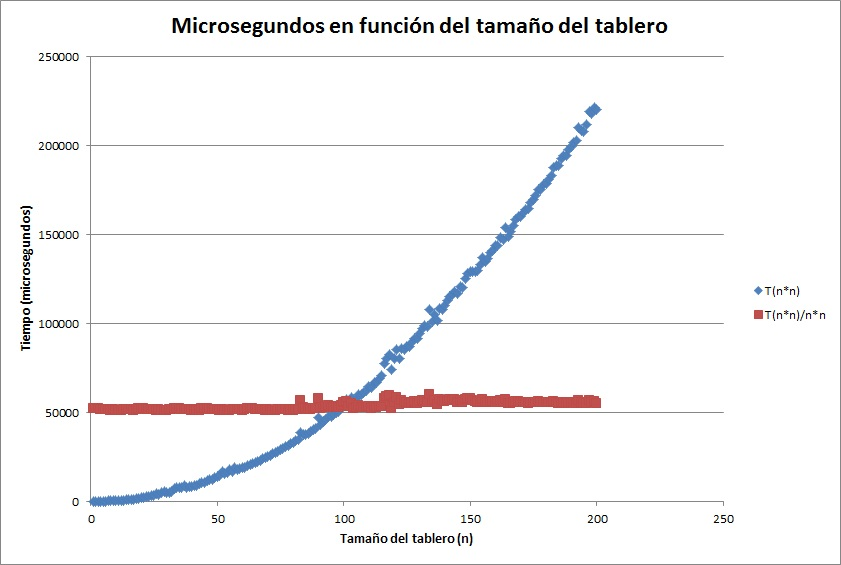
\includegraphics[scale=1]{Imagenes/Ej2/kFijo}
                \caption{T(n$^{2}$)=tiempo para tablero de tamaño n}
                \label{fig:exp2}
\end{figure} 
Como conclusión podemos ver que al dejar el k como una constante obtenemos una complejidad cuadrática del algoritmo contrastada en el gráfico.\\


Por ultimo una comparación cuando k y n varían de la misma manera con una cantidad de 300 instancias

\begin{figure}[H]
                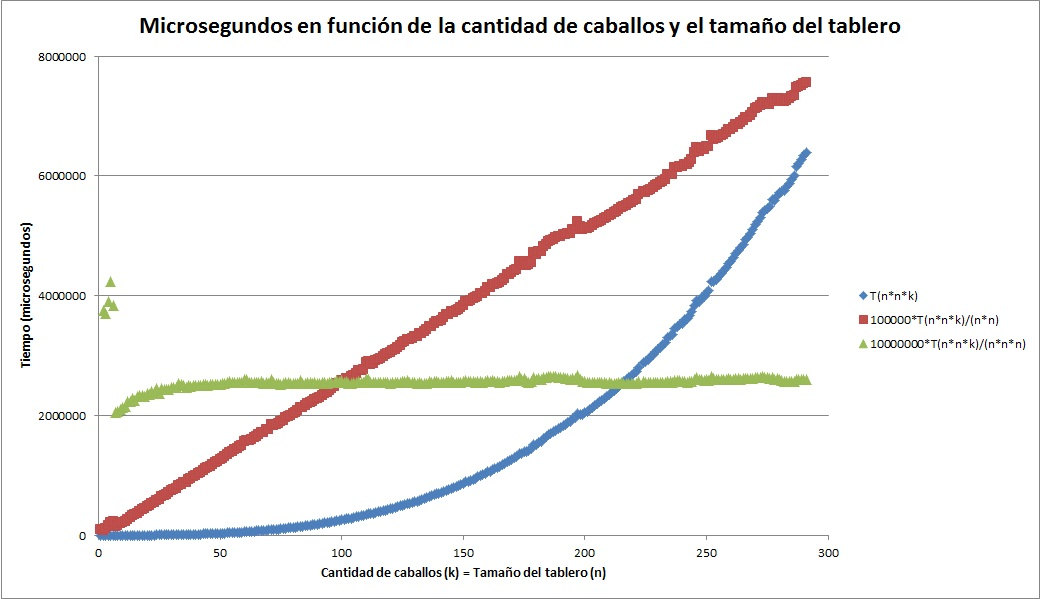
\includegraphics[scale=0.8]{Imagenes/Ej2/nkIguales}
                \caption{T(n$^{2}$*k)=tiempo para tablero de tamaño n = tiempo para k caballos}
                \label{fig:exp2}
\end{figure} 

En este último caso, se puede verificar una complejidad de O(n*$^{2}$*k)





\subsection{Conclusión}

Este ejercicio nos enseñó la posibilidad de utilizar algoritmos que a comienzo sirven para el recorrido de un grafo (BFS) como una manera de calcular caminos mínimos de grafos no pesados, o con todas las aristas del mismo peso. Con respecto al desarrollo, a priori no se nos presentó una dificultad al resolverlo, contamos con varias estrategias para encararlo, una de ellas era resolverlo con k matrices distintas para tener en cada matriz el camino mínimo a todas las casillas de un caballo nada más. Además pudimos cumplir con la complejidad que nos delimitaban y corroboramos empíricamente que el tiempo del algoritmo cumplía con esta.



